\setcounter{page}{1}
\section*{Zielsetzung}
Im Versuch 602 sollen Röntgenemissions- und Absorptionsspektren quantitativ untersucht werden.
Dies ermöglicht grundlegende Aussagen über den Atomaufbau und insbesondere die Energieniveaus
der betrachteten Stoffe.
\section{Theorie}
Als Röntgenstrahlung wird elektromagnetische Strahlung im Energiebereich $\SI{8}{\kilo\eV}$
bis $\SI{100}{\kilo\eV}$ bezeichnet. Röngenstrahlung befindet sich daher energetisch betrachtet oberhalb des sichtbaren Lichtes und
unterhalb von $\gamma$-Strahlung. Die hohe Energie ermöglicht eine Untersuchung von niedrigen Energieniveaus.
\subsection{Emission}
Zur Erzeugung von Röngenstrahlung wird eine Röntgenröhre nach Abbildung \ref{fig: röhre} verwendet. In einem
evakuierten Behälter werden aus einem Glühdraht Elektronen emittiert (Glühelektrischer Effekt) und durch eine
anliegende Spannung $U\ua{B}$ zu einer Kupferanode beschleunigt. Durch das Auftreffen an der Anode
entsteht die Röngenstrahlung. Hierbei setzt sich das entstehene Strahlungsspektrum aus zwei
Bestandteilen zusammen.\\
\begin{figure}
  \centering
  \includegraphics[width = 0.7\textwidth]{pics/röhre.png}
  \caption{Schematische Darstellung einer Röntgenröhre\cite{anleitung602i}.}
  \label{fig: röhre}
\end{figure}
Durch die Wechselwirkung mit dem Coulombfeld der Kerne des Anodenmaterials werden die Elektronen abgebremst. Da beschleunigte Ladungen strahlen,
wird bei diesem
Vorgang ein Röntgenquant ausgesendet, dessen Energie $E\ua{ph} = h\nu$ genau dem Energieverlust des Elektrons
entspricht. Das hierdurch entstehende Spektrum ist kontinuierlich, da das Elektron auch nur Teile seiner
Energie verlieren kann. Die Maximale Energie der Photonen $E\ua{ph, max}$ wird dann erreicht,
wenn ein Elektron gänzlich abgebremst wird
\begin{equation}
  E\ua{ph, max} = \frac{h c}{\map{e}\ua{0}U\ua{B}}.
  \label{eq: E_max}
\end{equation}
Es sind $h=\SI{6.626e-34}{\joule\second}$ das Plancksche Wirkungsquantum, $e\ua{0}=\SI{-1.602e-19}{\coulomb}$ die Elementarladung und
$c=\SI{299792458}{\meter\per\second}$ die Vakuumlichtgeschwindigkeit.
Das sogenannte charakteristische Röntgenspektrum entsteht durch Ionisation des Anodenmaterials.
Wird ein Elektron aus einer der unteren Schalen ionisiert, rückt ein Elektron unter Aussendung eines
Photons, dessen Energie $E\ua{ph}$ genau der Energiedifferenz zwischen den Schalen entspricht, in die Fehlstelle nach.
\begin{equation}
  E\ua{ph} = h\nu = \frac{h c}{\lambda} = E\ua{m} - E\ua{n}.
  \label{eq: photonenenergie}
\end{equation}
Die Ionisation kann nur dann stattfinden, wenn die Energie des Elektrons mindestens der Ionisationsenergie der betreffenden Schale entspricht.
Das Spektrum weist daher für das Anodenmaterial charakteristische diskrete Linien auf. Die Linien werden durch zwei Buchstaben
gekennzeichnet. Der erste gibt die Schale ($K$, $L$, $M$ usw.) an, aus der ein Elektron ausgelöst wird, der zweite Buchstabe
($\alpha$, $\beta$ usw.) zeigt auf aus welcher höheren Schale ein Elektron nachgerückt. So kennzeichnet etwa
$K\ua{\alpha}$ die Linie, die entsteht, wenn ein Elektron aus der $K$-Schale ionisiert wird und ein Elektron aus der $L$-Schale
nachrückt. Für die Bindungsenergien $E\ua{n}$ gilt
\begin{equation}
  E\ua{n} = -R\ua{\infty} z\ua{eff}^2 \frac{1}{n^2}.
  \label{eq: E_niveaus}
\end{equation}
Hierbei entspricht $R\ua{\infty} = \SI{13.6}{\eV}$ der Rydbergenergie und $z\ua{eff}$ der effektiven Kernladung. Die effektive
Kernladung berücksichtigt die Abschirmung des Coulombpotentials in einem Mehrelektronenatom. Es gilt näherungsweise
\begin{equation}
  z\ua{eff} = z - \sigma\ua{n}.
  \label{eq: abschirmkonstante}
\end{equation}
Mit der Kernladung $z$ und der Abschirmkonstante $\sigma\ua{n}$, deren Wert für alle Elektonen einer Schale als konstant angenommen wird.
Für die Energie der $K\ua{\alpha}$-Linie gilt damit
\begin{equation}
  E\ua{K\ua{\alpha}}(\sigma_1, \sigma_2) = R\ua{\infty} \left[\left(z - \sigma_1\right)^2 -  \frac{1}{4}\left(z - \sigma_2\right)^2\right].
  \label{eq: E_K_alpha}
\end{equation}
Entsprechend ergibt sich $E\ua{K\ua{\beta}}$ zu
\begin{equation}
  E\ua{K\ua{\beta}}(\sigma_1, \sigma_3) = R\ua{\infty} \left[\left(z - \sigma_1\right)^2 -  \frac{1}{9}\left(z - \sigma_3\right)^2\right].
  \label{eq: E_K_beta}
\end{equation}
Um Audrücke für die Abschirmkonstanten $\sigma_1$ und $\sigma_2$ zu erhalten wird diese Energiedifferenz
näherungsweise mit der Ionisierungsenergie $E\ua{K}$ gleichgesetzt.
\begin{align}
  \begin{aligned}
  E\ua{K\ua{\beta}}(\sigma_1, \sigma_3) &\approx E\ua{K}(\sigma_1) = R\ua{\infty} \left(z - \sigma_1\right)^2 \\
  \Rightarrow \quad \sigma_1 &= z - \sqrt{\frac{E\ua{K\ua{\beta}}}{R\ua{\infty}}}.
  \label{eq: sigma_1}
\end{aligned}
\end{align}
Die Lösung mit positivem Vorzeichen ist unphysikalisch und wird ignoriert. Einsetzen in \eqref{eq: E_K_alpha} ergibt für $\sigma_2$
\begin{equation}
  \sigma_2 = z - 2\sqrt{\frac{ E\ua{K\ua{\beta}} - E\ua{K\ua{\alpha}} }{ R\ua{\infty} } }.
  \label{eq: sigma_2}
\end{equation}

Es ist weiter zu beachten, dass die Elektronen eines Energieniveaus
aufgrund des individuellen Bahndrehimpulses bzw. Spins nicht alle die selbe Ionisierungsenergie besitzen. Daher verfügt das charakteristische
Spektrum für Schalen mit mehr als einem Elektron über eine Feinstruktur eng beieinander liegender Linien.

\subsection{Absorption}
Die Absorption von Röntgenstrahlung wird im Wesentlichen durch den Photo- und den Comptoneffekt hervorgerufen.
Als Photeffekt wird das Auslösen eines in einem Atom gebundenen Elektrons unter Absorption eines Photons bezeichnet. Die
Energie des einfallenden Photons muss also mindestens der Bindungsenergie des Elektrons entsprechen.
Aufgrund der hohen Strahlungsenergie kann der Photoeffekt insbesondere durch Wechselwirkung mit Elektronen der unteren
Schalen stattfinden (innerer Photoeffekt). Der Compton-Effekt, der den Energieverlust der Röngenquanten duch Wechselwirkung
mit schwach gebundenen Elektronen beschreibt (quasi-freie Teilchen), bewirkt gemäß den Gesetzen des elastischen Stoßes
einen kleinen Energieverlust bzw. Richtungsänderungen.
Hierdurch wird das Spektrum in seiner Intensität abgeschwächt.
Die Absorption
fällt monoton mit steigender Energie der Röntgenstrahlung. Bei diskreten Energien kommt es jedoch sprunghaft zu einem Anstieg. Diese
sogenannten Absorptionskanten treten genau bei den Ionisierungsenergien der Energieniveaus auf.
Graphik \ref{fig: absorption} zeigt einen charakteristischen
Verlauf der Absorption unter variabler Wellenlänge ($E \propto \frac{1}{\lambda}$) der einfallenden Strahlung.
Die Absorptionskanten werden entsprechend der Schale bezeichnet, die ionisiert wird. Die Untersuchung der Lage der Kanten
ermöglicht eine Bestimmung der Ionisierungsenergien bzw. der Abschirmkonstanten.
Auch hier ist die Feinstruktur zu beachten, die dazu
führt, dass für Schalen mit mehr als einem Elektron mehrere Kanten zu beobachten sind (z.B. $L\ua{I}$, $L\ua{II}$, $L\ua{III}$).
Die Kanten $L\ua{I}$ und $L\ua{II}$ können in diesem Versuch nicht aufgelöst werden. Eine Untersuchung der Energiedifferenz
$\Delta E\ua{L} = E\ua{L\ua{II}} - E\ua{L\ua{III}}$ ermöglicht gemäß folgender Formel eine Bestimmung der Abschirmkonstanten
$\sigma\ua{L}$ der $L$-Schale
\begin{equation}
  \sigma\ua{L} = z - \left\{ \left(\frac{4}{\alpha}\sqrt{\frac{\Delta E\ua{L}}{R\ua{\infty}}} -\frac{5\Delta E\ua{L}}{R\ua{\infty}} \right)
  \left(1 + \frac{19}{32}\alpha^2\frac{\Delta E\ua{L}}{R\ua{\infty}} \right)  \right\}^{1/2}.
  \label{eq: sigma_L}
\end{equation}
\begin{figure}[H]
  \centering
  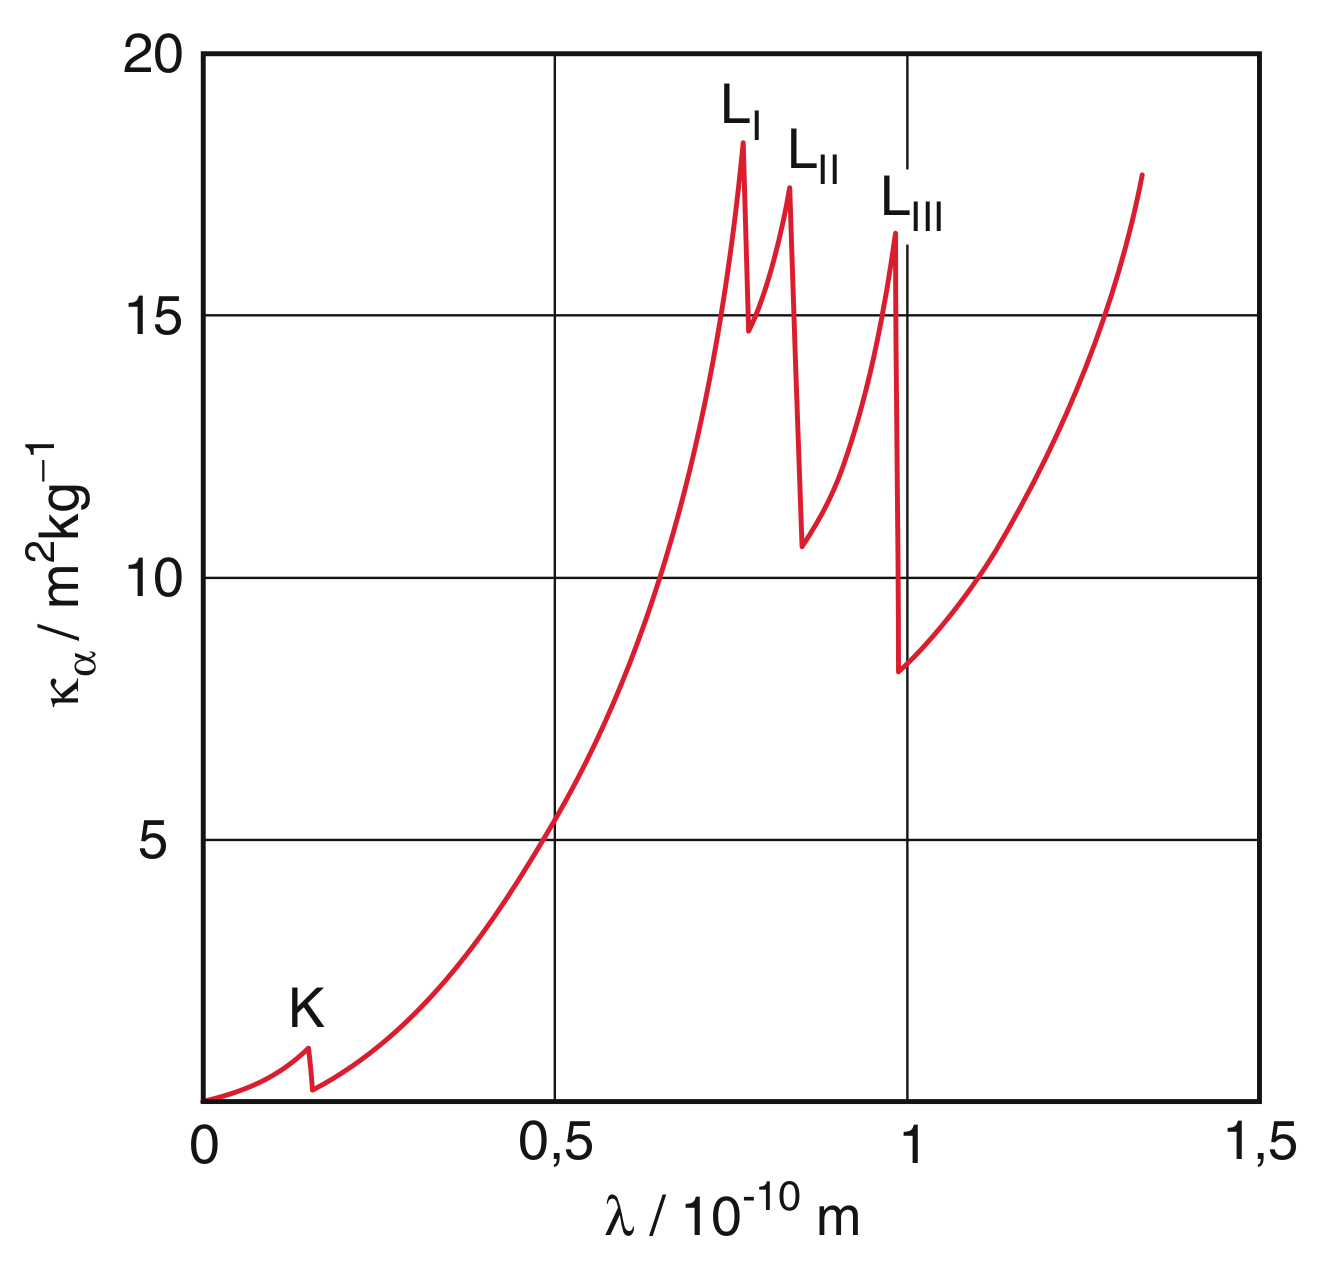
\includegraphics[width = 0.4\textwidth]{pics/absorption.png}
  \caption{Charakteristisches Röntgenabsorptionsspektrum für Blei\cite{dem}.}
  \label{fig: absorption}
\end{figure}

\subsection{Bragg-Bedingung}
Zur Analyse des Röntgenenergiespektrums wird ausgenutzt, dass die Beugung elektromagnetischer Strahlung an kristallinen
Oberflächen von der Wellenlänge abhängt. Für die $n$-te Beugungsordnung gilt nach der Bragg-Bedingung
\begin{equation}
  2 d \sin\theta = n \lambda.
  \label{eq: bragg}
\end{equation}
Hierbei entspricht $d$ der Gitterkonstanten und $\theta$ dem Glanzwinkel. Damit lässt sich jedem Winkel $\theta$ eindeutig eine
Energie der am Gitter gebeugten Photonen zuordnen
\begin{equation}
  E(\theta) \overset{\eqref{eq: photonenenergie} }{\underset{n = 1}{=}} \frac{h c}{2 d \sin \theta}.
  \label{eq: E_beugungswinkel}
\end{equation}
